\section{Technical Tools} \label{ch:methods:tech}

\subsection{Striatal Lesion} \label{ch:method:lesion}
\begin{figure}[bth!]
	\begin{center}
		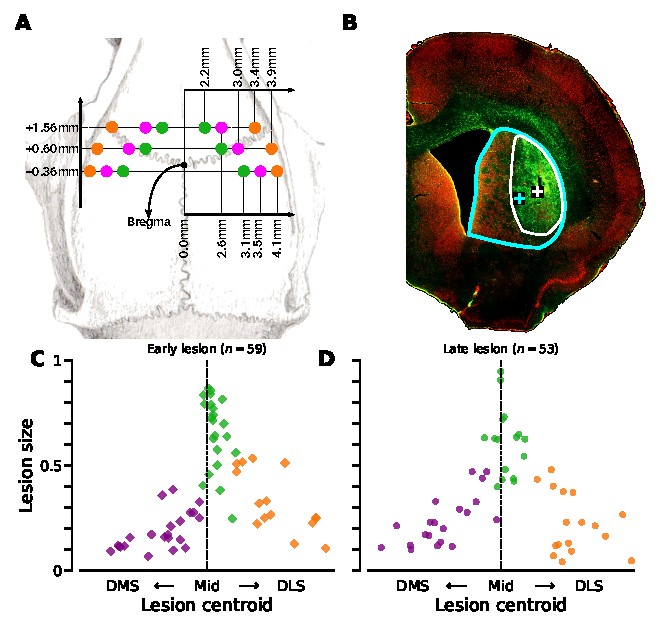
\includegraphics[scale=1]{ch-methods/figures/LesionSizeLocation.pdf}
		\caption
		{\textbf{Dorsal striatum lesion quantification.}
		\textbf{A)} Schematic of the lesion sites.
		\textbf{B)} Illustration of the quantification of the lesion size.
		For each coronal slide and hemi-striatum, the contour of the lesion was manually outlined using the GFAP staining.
		The relative size of the lesion (compared to the full striatum, manually outlined on the NeuN staining) and the coordinates of the lesion/striatum centroid was calculated.
		For each animal, the size and laterality were obtained by averaging data along the anteroposterior axis, for both left and right hemispheres.
		\textbf{C, D)} Lesion size versus laterality for animals that underwent lesion before (Early, \textbf{C}) and after (Late, \textbf{D}) extensive practice.
		Lesion quantification was performed blindly relative to behavioral analysis.
		In four animals with a striatal lesion performed after learning the task (late lesion), the lesion size quantification could not be properly performed.
		These animals were classified according to their injection coordinates in the surgery (3 DLS and 1 DMS), however they were excluded from any analysis that required the lesion size (hence the difference between the number of ``late lesion'' animals in this figure, $n=53$, and the total number of animals in \autoref{fig:lesion:task}, $n=57$).
		}
		\label{fig:method:LesionSizeLocation}
	\end{center}
\end{figure}


\subsection{Statistics}
All statistical comparisons were performed using a permutation test previously described in~\cite{Fujisawa2008NN}.
This non-parametric method alleviates many concerns in statistical hypothesis tests, such as distribution assumptions (e.g., normality assumption under analysis of variance), error inflation due to multiple comparisons, and sensitivity to unbalanced group size.
\par
To simplify the description, let's assume, we have ${\mathbf{X}=[X_1, X_2,...,X_n]}$, where $X_i$ is the set of $ET$s of session~$i$.
Similarly, we have $\mathbf{Y}$ that contains \glspl{et} of all the sessions from another condition.
Here, the null hypothesis states that the assignment of each data point in $X_i$ and $Y_i$ to either $\mathbf{X}$ or $\mathbf{Y}$ is random, hence there is no difference between $\mathbf{X}$ and $\mathbf{Y}$.
\par
In short, the test statistic was defined as the difference between smoothed (using Gaussian kernel with $\sigma =0.05$) $\mathbf{X}$ and $\mathbf{Y}$ for each session~$i$: $D_0(i)$.
At this point, we generated one set of surrogate data by assigning each \gls{et} of session $i$ to either $X_i$ or $Y_i$, randomly.
For each set of surrogate data, the test statistic was calculated, i.e.,~$D_m(i)$.
This process was repeated 10,000 times for all the statistical comparisons in this study, obtaining: $D_1(i),\ldots,D_{10000}(i)$.
\par
At this step, two-tailed pointwise p-values could be directly calculated for each $i$, from the $D_m(i)$ quantiles~\cite[see][]{Fujisawa2008NN}.
Moreover, to compensate for the issue of multiple comparisons, we defined global bands of significant differences along the session index dimension.
From 10,000 sets of surrogate data, band of the largest $\alpha$-percentile was constructed, such that less than 5\% of $D_m(i)$s broke the band at any given session $i$.
This band (denoted as the \textit{global band}) represents the threshold for significance, and any break-point by $D_0(i)$ at any $i$ is a point of significant difference between $\mathbf{X}$ and $\mathbf{Y}$.
\par
In cases of comparing only two sets of data points, the same algorithm was employed, having only one value for index $i$.
If none of the $D_m(i)$s exceeded $D_0(i)$, the value $p<0.0001$ was reported (i.e., less than one chance in 10,000).
